\chapter{Technical equipment}

\section{Inertial measurement unit}
Inertial measurement unit (IMU) data, an inertial measurement unit (IMU), usually refers to a combined unit consisting of three accelerometers and three gyroscopes mounted on mutually perpendicular measurement axes.\cite{iosa2016wearable} Inertial sensors including accelerometers (or accelerometer sensors) and angular velocity sensors (gyros) and their single, dual, and triaxial combinations IMU (Inertial Measurement Unit), AHRS (Attitude Reference System including magnetic sensors). IMU sensors are used in everyday life, smartphones, smartwatches, and commercial drones, among other electronic products. Commercially available off-the-shelf IMU sensors are small, lightweight, wireless devices that IMU sensors can quickly fix to a body part without interfering with motion. Depending on their application, they are typically embedded in Bluetooth/wireless transmitters or SD cards for real-time data streaming or onboard long-term data recording, respectively.
\begin{figure}[htbp]
\centering
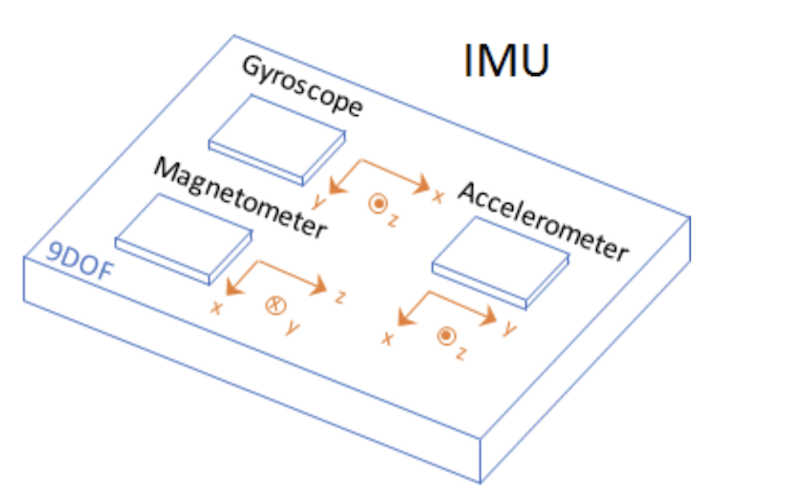
\includegraphics[width=9cm]{report/pics/IMU Sensor .png}
\caption{IMU Sensors' internal structure includes an accelerometer, Magnetometer, and gyroscope.\cite{IMU} }
\end{figure}\\
\section{Working Principle}
 An IMU sensor unit working can be done by using one or more accelerometers to detect linear acceleration and similarly by using gyroscopes to detect rotation rates and magnetometers. \cite{hazry2009study}
 
 
 \section{IMU sensors in our work}
Nowadays, wearable IMU sensors are widely used in medical research, and the acceleration data collected by IMU helps to predict and analyze patient data in the future. Wearable IMU sensors will collect daily data from Parkinson's patients in our present work. We will collect acceleration and angular acceleration from the wrists, ankles, and other body parts of people with Parkinson's disease. We use the MJFF Levodopa wearable sensor dataset \cite{MJFF}, and the Fox Foundation collects wearable sensor data from patients with Parkinson's disease (PD). Subjects were recruited from two clinical sites and monitored while performing a range of routine activities in the clinic and daily activities at home. In Chapter 5, we describe the data collection information in detail.\\

\begin{figure}[htbp]
\centering
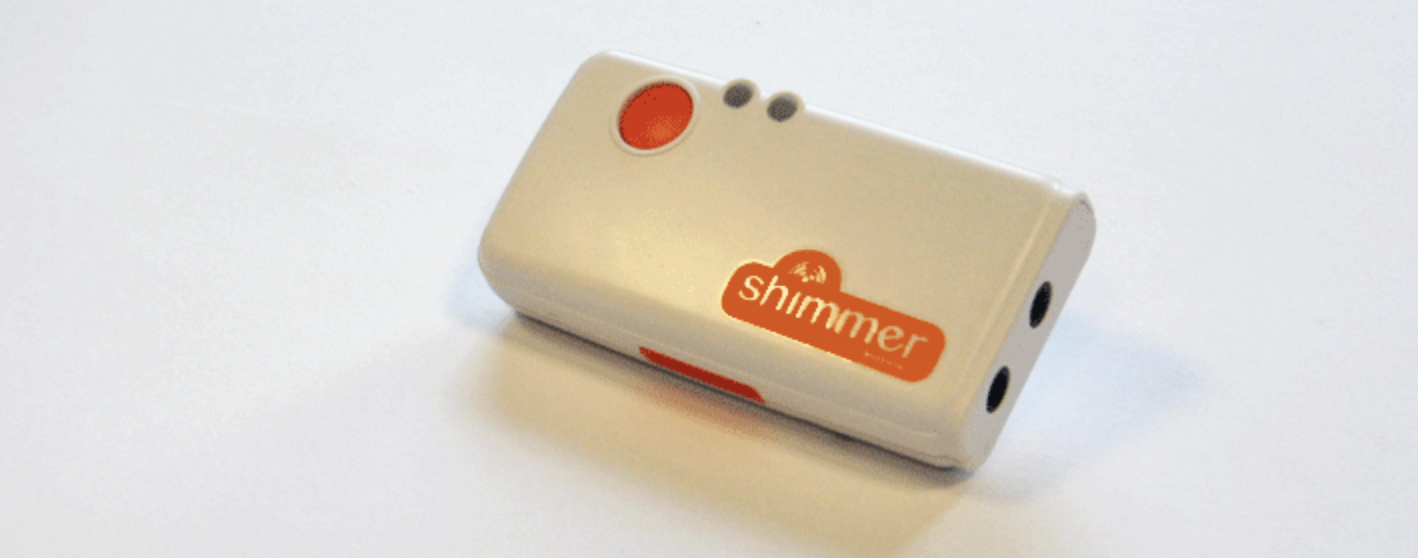
\includegraphics[width=9cm]{report/pics/Shimmer Sensor.png}
\caption{Shimmer3 offers the best data quality with integrated 9DoF inertial sensing via accel, gyro, mag, and pressure sensor, each with selectable range.} \cite{ShimmerSensor}
\end{figure}
The Shimmer sensor is used in medical, neuroscience, and clinical research and is a highly accurate IMU sensor. The Shimmer IMU comes with integrated 9 DoF + altimeter inertial sensing via accelerometer, gyroscope, and magnetometer, each with a selectable range.\cite{ShimmerSensor} But the shimmer sensor is not cheap. Just one Shimmer sensor needs to spend 598 euros. The truth is that IMU sensors are ubiquitous in our lives, such as cell phones and smartwatches. So it is better value for money to wear a watch and a cell phone than to wear a professional IMU sensor.
